%!TEX root = interval-interdiction-ciac.tex
% This is the version after considering empty intervals = isolated vertices

\newcommand{\scat}{\text{sc}}

\section{Scattering Number, Hamiltonicity, and Graph Toughness}
\label{sec:hamiltonicity}
In this section, we \las{investigate the shrink-expand framework with respect to various parameters related to Hamiltonicity of an interval graph. All the problems considered in this section are of the same structure: As input we are given an interval graph in the shrink-expand framework with shrinking intervals. The given graph is Hamiltonian (or has a property similar to Hamiltonicity, like a Hamilton path, a small path cover, large graph toughness), and the question is whether the interdictor can destroy this property by shrinking at most $k$ intervals for a given budget $k$. In this section, we consider interdiction problems and most vital nodes problems with respect to Hamilton cycle, Hamilton path, path cover (\cref{subsection:ham_interdict,subsection:ham_mvn}), and graph toughness (\cref{subsection:tough}), as well as the assistance problem for scattering number (\cref{subsection:scat}). The formal definition of each of these problems is given at the beginning of the corresponding subsection. We show that each of these problems can be solved in polynomial time.}

\las{Before we begin, we have to introduce the concept of the \emph{scattering number}, which is crucially related to Hamiltonicity of interval graphs.}
We define by $c(G)$ the number of connected components in a graph $G$.
The scattering number of a graph $G$, denoted by $\scat(G)$, was defined by Jung~\cite{jung1978scat} as follows:

\[
    \scat(G) := \max \{c(G-S) - |S| : S \subseteq V(G) \text{ and } c(G-S) > 1\}.
\]
If the set above is empty, the graph $G$ is a complete graph, and in this case, we define $\scat(G) = -\infty$.

For an interval graph, the scattering number characterizes the Hamiltonicity of the graph, as summarized in the following theorem:

\begin{theorem}[Deogun, Kratsch, and Steiner~\cite{deogun1997scat}]
\label{thm:scat}
For an interval graph $G$ and for all constants $p \geq 1$,
\begin{itemize}
	\item $G$ contains a Hamilton path, if and only if $\scat(G) \leq 1$;
	\item $G$ contains a Hamilton cycle, if and only if $\scat(G) \leq 0$;
	\item $G$ contains a path cover of size $p$, if and only if $\scat(G) \leq p$.
\end{itemize}
\end{theorem}

One can easily see that the ``$\Rightarrow$" directions in the above theorem are true for any graph. In this section, we will prove the following theorem: (the formal definitions of the problems will be presented in the later subsections)

\begin{theorem}
\label{thm:ham}
In the shrink-expand framework, the following problems can be solved in time $\bigO(kn^3)$:
\begin{itemize}
	\item[(a)] The assistance problem for scattering number,
	\item[(b)] The interdiction problem for Hamilton path,
	\item[(c)] The interdiction problem for Hamilton cycle,
	\item[(d)] The interdiction problem for path cover,
\end{itemize}
\end{theorem}

As the scattering number is the central parameter in this section, we will first present the method to solve \las{the} assistance problem for scattering number in Section~\ref{subsection:scat}.
After that, we will show how by solving this problem, we can solve the interdiction problems mentioned in Theorem~\ref{thm:ham}.

We also discuss briefly two implications of the above theorem. 
Firstly, in Section~\ref{subsection:ham_mvn}, we show how the most vital nodes problem for Hamiltonicity parameters can be reduced to the assistance problem for scattering number and hence can be solved in similar time. 
Secondly, the method to solve the above assistance problem can be easily extended to the interdiction problem of a related parameter, graph toughness. 
In Section~\ref{subsection:tough}, we will define this parameter and discuss the modification needed to apply the method above to solve the latter problem. 

\subsection{Assistance Problem for Scattering Number}
\label{subsection:scat}

The assistance problem for $\scat(G)$ is to compute $\max_{|X| \leq k}\scat(G_X)$ with shrinking intervals. 
In other words, we want to compute 

\begin{equation}
\label{eq:scat_assist}
  \max_{X \subseteq [n], |X| \leq k} \, \max_{S \subseteq [n], c(G_X - S) > 1} c(G_X - S) - |S|.
\end{equation}

We interprete problem (\ref{eq:scat_assist}) as a cooperative two-player game between an \emph{assistant} and the network owner. 
The assistant first selects the indices $\las{X \subseteq [n]}$ of the intervals to shrink, obtaining some graph $G_X$. 
After that, the network owner selects a set $\las{S \subseteq [n]}$ of vertices in $G_X$. 
The goal is that the property $c(G_X - S) > 1$ holds, and that under this condition, the value $c(G_X - S) - |S|$ is as large as possible.
\las{The goal of this subsection is to show that the optimal strategy of this game can be computed efficiently, i.e.\ we show that expression~(\ref{eq:scat_assist}) can be evaluated in polynomial time.
Since the argument is involved, we split it into several parts. We first briefly sketch the main idea without giving too many details.
After that, we introduce a certain important non-deterministic process used for the proof and explain the intuition behind it. Finally, we give a formal proof.}

\subsubsection{\las{The idea.}}

\las{We briefly sketch the main idea behind the proof. First, observe that we can w.l.o.g.\ assume that $X \cap S = \emptyset$. Indeed, whenever we have some number $i \in X \cap S$, it means that  the corresponding interval gets shrunk by the first player, and then deleted by the second player. But if a deletion occurs anyway, shrinking the interval is unnecessary for the goal of maximizing $c(G_X - S)$. This motivates}
 the following definition: A pair $(X,S)$ with $X, S \subseteq [n]$ is called a \emph{candidate pair}, if $|X| \leq k$ and $X \cap S = \emptyset$.
Further, we define 
\[
s(X,S) := \begin{cases} 
c(G_X - S) - |S| &\text{if } c(G_X - S) > 1,\\ 
-\infty &\text{otherwise.}
\end{cases}
\]
By the above explanations, we then have that the value of expression (\ref{eq:scat_assist}) is exactly 
\begin{equation}
 \max_{(X, S) \text{ candidate pair}} s(X, S). \label{eq:scat_assist_prime}
\end{equation}

\las{So it suffices to compute expression~(\ref{eq:scat_assist_prime}). How can we do that? 
We will introduce a non-deterministic process, which we call \emph{process $P$}. 
This process takes as input the instance $(\I, \I', k)$ and outputs some non-deterministically chosen value $\beta$. 
The idea behind this process $P$ is to mimic the cooperative game between the assistant and the network owner, but restrict it to certain rules, which preserve ``locality" during the process. 
The property that $P$ is non-deterministic corresponds to the fact that the two players have multiple choices during their game. 
The idea is that the output $\beta$ is ``the same" as the number $s(X,S)$, and so it is desirable to take those non-deterministic choices during a run of $P$ that maximize the output value $\beta$. 
 In the remainder of the subsection, we will first describe $P$ formally and provide an intuition for all its components. 
We will then prove our central lemma (\cref{lem:process_P}). It states that if $\beta_\text{max}$ is the maximum value that is returned by some run of $P$, then $\beta_\text{max}$ is equal to expression~(\ref{eq:scat_assist_prime}). 
Our second lemma (\cref{lem:ham_path}) states that $\beta_\text{max}$ can be computed in polynomial time using a dynamic program. Therefore, once we have proven these lemmas, we have shown that expressions~(\ref{eq:scat_assist_prime}) and (\ref{eq:scat_assist}) can be evaluated in polynomial time, as desired.}


\subsubsection{\las{The process $P$.}}

\SetKw{KwDownTo}{down to}
\SetKwBlock{KwBeginAA}{1a.)}{end}
\SetKwBlock{KwBeginAB}{1b.)}{end}
\SetKwBlock{KwBeginBA}{2a.)}{end}
\SetKwBlock{KwBeginBB}{2b.)}{end}
\SetKwBlock{KwBeginBC}{2c.)}{end}
\begin{algorithm}[htpb]
\color{blue}
 \KwIn{Sequences $\I = ([a_1,b_1], \dots, [a_n,b_n])$ and $\I' = ([a'_1,b'_1], \dots, [a'_n,b'_n])$ s.t.\ $\forall i \in \set{1,\dots,n}: a_i \leq a'_i \leq b'_i \leq b_i \ $. Integer $k \geq 0$.}
 \KwOut{A non-deterministically chosen value $\beta$.}
 $\mathcal{F} = \I \cup \I' = \fromto{[c_1,d_1]}{[c_{2n},d_{2n}]}$ ordered by endpoint, i.e.\ $d_1 < d_2 < \dots < d_{2n}$ (w.l.o.g. $d_i \neq d_j$ for $i \neq j$). Let $F_i := [c_i, d_i]$ for $i \in \fromto{1}{2n}$.\;
 $k' \gets k$, $\gamma \gets 0$, $\beta \gets 0$\;
 $L \gets \emptyset$ \tcp*{stored using two variables, i.e. $L= [\ell, r]$}
\For{$i \gets 2n$ \KwDownTo $1$}{
	\eIf{$F_i \in \I$} {
		Let $t \in [n]$ s.t. $F_i = I_t$\;
		Choose non-deterministically exactly one of 1a.) or 1b.)\\
		\KwBeginAA{
			 $\textsc{lock}(I_t)$\; 
			\eIf{$I_t \cap L \neq \emptyset$}{
				$L \gets L \cup I_t$\;
			}
			{
				$L \leftarrow I_t$\;
				$\beta \gets \beta + 1$\;
				$\gamma \gets \min\{\gamma + 1, 2\}$\;
			}
		}
		\KwBeginAB{
			$\textsc{delay}(I_t)$\;
		}
	}
	{
		In this case we have $F_i \in \I'$. Let $t \in [n]$ s.t. $F_i = I'_t$. Choose non-deterministically exactly one of 2a.) or 2b.) or 2c.), subject to the constraints listed below.\\
		\KwBeginBA{
			Constraint: Only choosable if $I_t \subseteq L$\;
			$\textsc{lock}(I_t)$, $\textsc{discard}(I'_t)$\;
		}
		\KwBeginBB{
			Constraint: Only choosable if $I_t \not\subseteq L$\;
			$\textsc{delete}(I_t)$, $\textsc{discard}(I'_t)$\;
			$\beta \leftarrow \beta - 1$\;
		}
		\KwBeginBC{
			Constraint: Only choosable if $k' > 0$ and $I_t \not\subseteq L$\;
			$\textsc{shrink}(I_t)$, $\textsc{lock}(I'_t)$\;
			$k' \leftarrow k' - 1$\;
			\eIf{$I'_t \cap L \neq \emptyset$}{
				$L \gets L \cup I'_t$\;
			}
			{
				$\beta \gets \beta + 1$\;
				$\gamma \leftarrow \min\{\gamma + 1, 2\}$\;
				\lIf{ $I'_t \neq \emptyset$}{
					$L \leftarrow I_t'$ \label{algline:empty}
				}
			}
		}
	}
}
\leIf {$\gamma < 2$}{\KwRet{$- \infty$}}{\KwRet{$\beta$}}

 \caption{The non-deterministic process $P$.}
 \label{alg-chapter-4}
\color{black}
\end{algorithm}
%%%%%%%%%%%%----------------------
\las{Consider Algorithm~\ref{alg-chapter-4}, which provides a complete description of $P$ in pseudo-code. Before we proceed with the formal proof of our main lemmas, we explain in this paragraph the ideas behind process $P$ and its components.}

\las{Process $P$ receives as input an integer $k \geq 0$ and sequences of intervals $\I = (I_1,\dots,I_n) = ([a_1,b_1], \dots, [a_n,b_n])$ and $\I' = (I'_1,\dots,I'_n) = ([a'_1,b'_1], \dots, [a'_n,b'_n])$, such that for all $i \in \set{1,\dots,n}$ we have $a_i \leq a'_i \leq b'_i \leq b_i$. We can assume w.l.o.g.\ that $a_i < b_i$ for all $i=1,\dots,n$. However, a special case that we cannot avoid is that for some indices $i$ it could be the case that $a'_i = b'_i$. Recall that we defined in the introduction that in this case we have $[a'_i, b'_i] = \emptyset$. (This definition may seem a bit unorthodox. However, it is crucial to correctly model the most vital nodes problem later in \cref{subsection:ham_mvn}.)
}

\las{After $P$ has received its input, it considers the union $\mathcal{F} := \I \cup \I'$ and orders it by the endpoints of the intervals, i.e.\ $\mathcal{F} = \fromto{F_1}{F_{2n}} = \fromto{[c_1,d_1]}{[c_{2n},d_{2n}]}$ such that $d_1 < d_2 < \dots < d_{2n}$ (we can w.l.o.g. assume that no two endpoints are equal). The main idea of $P$ is now to consider all the intervals $F_i$, starting with $i=2n$ and going down towards $i=1$, and making a partial decision about the fate of interval $F_i$. In particular, this decision is indicated by some keywords,  $\textsc{shrink}, \textsc{lock}, \textsc{delete}, \textsc{discard}, \textsc{delay}$. The meaning behind the keywords is as follows:}
Consider some index $t \in [n]$ and the pair of original interval $I_t$ and its replacement interval $I'_t$ with $I'_t \subseteq I_t$. 

\begin{itemize}
	\item[(i)] \las{Case 2c.) of the process: $\textsc{shrink}(I_t)$, $\textsc{lock}(I'_t)$ can be interpreted in the following way: It means that} the assistant \emph{shrinks} the original interval $I_t$ down to the replacement $I'_t$ and the network owner does \emph{not} delete the corresponding vertex $t$. We say that $I'_t$ gets \emph{locked}.
	\item[(ii)] \las{Case 2b.) $\textsc{delete}(I_t)$, $\textsc{discard}(I'_t)$ means that} the assistant does not shrink the original $I_t$, but the network owner \emph{deletes} the corresponding vertex $t$. We also say that the network owner \emph{deletes} $I_t$.
	\item[(iii)] \las{Case 1a.) or 2a.) $\textsc{lock}(I_t)$  means that the assistant decides not to shrink $I_t$, and the network owner decides not to delete the corresponding vertex $t$}.  We say that $I_t$ gets \emph{locked}. 
	\item[(iv)] \las{Case 1b.) $\textsc{delay}(I_t)$  means that neither the assistant nor the network owner want to decide on the fate of $I_t, I'_t$ right now. Instead the decision of what to do gets delayed into the future, when the process encounters $I'_t$. This option seems strange, but it turns out to be necessary in order to have a process with high ``locality".} 
	
\end{itemize}

\las{We will prove, that no interval is associated with two conflicting keywords, and every interval is associated with at least one keyword. This in turn implies that process $P$ can be understood as an alternative way to construct a candidate pair $(X, S)$.}
Note that for this pair $(X,S)$, the following holds: The interval representation of the graph $G_X - S$ consists of exactly those intervals $F \in \I \cup \I'$, for which $\textsc{lock}(F)$ has been called. In other words, locking an interval $F \in \I \cup \I'$ means committing to the final decision, that this interval will be part of (the interval representation of) $G_X - S$. 

\las{The concept of locking intervals is important for understanding the variable $L$. The variable $L$ is always an interval $L = [\ell, r]$, which is initially the empty interval. For the following explanation, we assume for the sake of simplicity that there are no indices $i$ with $a'_i = b'_i$.}
At each point in time $i = 2n, \dots, 1$ during the execution of $P$, let $R_i \subseteq \mathcal{F}$ be the set of \las{all the intervals in $\mathcal{F}$} that have been locked so far. The interval graph $\graph(R_i)$ has multiple components in general. Let $R_i' \subseteq R_i$ be the set of intervals corresponding to the leftmost component. \las{We will prove that process $P$} maintains two invariants: 
\begin{equation}
\label{eq:invariant_lock_in_alg}
L = \bigcup_{F \in R_i'}F \text{ and } r \geq d_i. 
\end{equation}
The first invariant essentially means that $L$ \las{at each point in time describes the space which the leftmost connected component of $G(R_i)$ occupies (note here that the union of intervals associated with one connected component in fact again is a single interval)}. The second invariant naturally follows the order of processing from largest endpoint to the smallest. \las{We remark that line~\ref{algline:empty} of the pseudo-code contains a special handling of the case where $a'_t = b'_t$. This special handling means that empty intervals do not interact with $L$.}

Finally, process $P$ \las{stores some variables in memory}, which are initialized at the start, and updated depending on the choices taken. One of these variables, $\beta$, will be such that its final value at the end of the process equals exactly $s(X, S)$. \las{This is because in line with the definition of $s(X,S)$, the variable $\beta$ is decreased every time we delete some interval, and increased every time we create a new connected component with the intervals $R_i$.} In addition, the process \las{stores} in memory a variable $k'$, which starts with value $k$ and describes the remaining budget of the assistant.
Finally, the process also keeps in memory a variable $\gamma$ that indicates $\min\{c(G(R_i)),2\}$.
In words, this variable keeps track of how many connected components are formed by the locked intervals so far.
Since at the end, we are only interested in whether the number of connected components is at least two, we cap the value of this variable at two.

\las{This completes our description of the process $P$.} Figure~\ref{fig:ham_path} contains an illustration of an execution of process $P$.
At the beginning, where $L = \emptyset$, we use the convention $\ell = r = \infty$. 
\begin{figure}
\centering
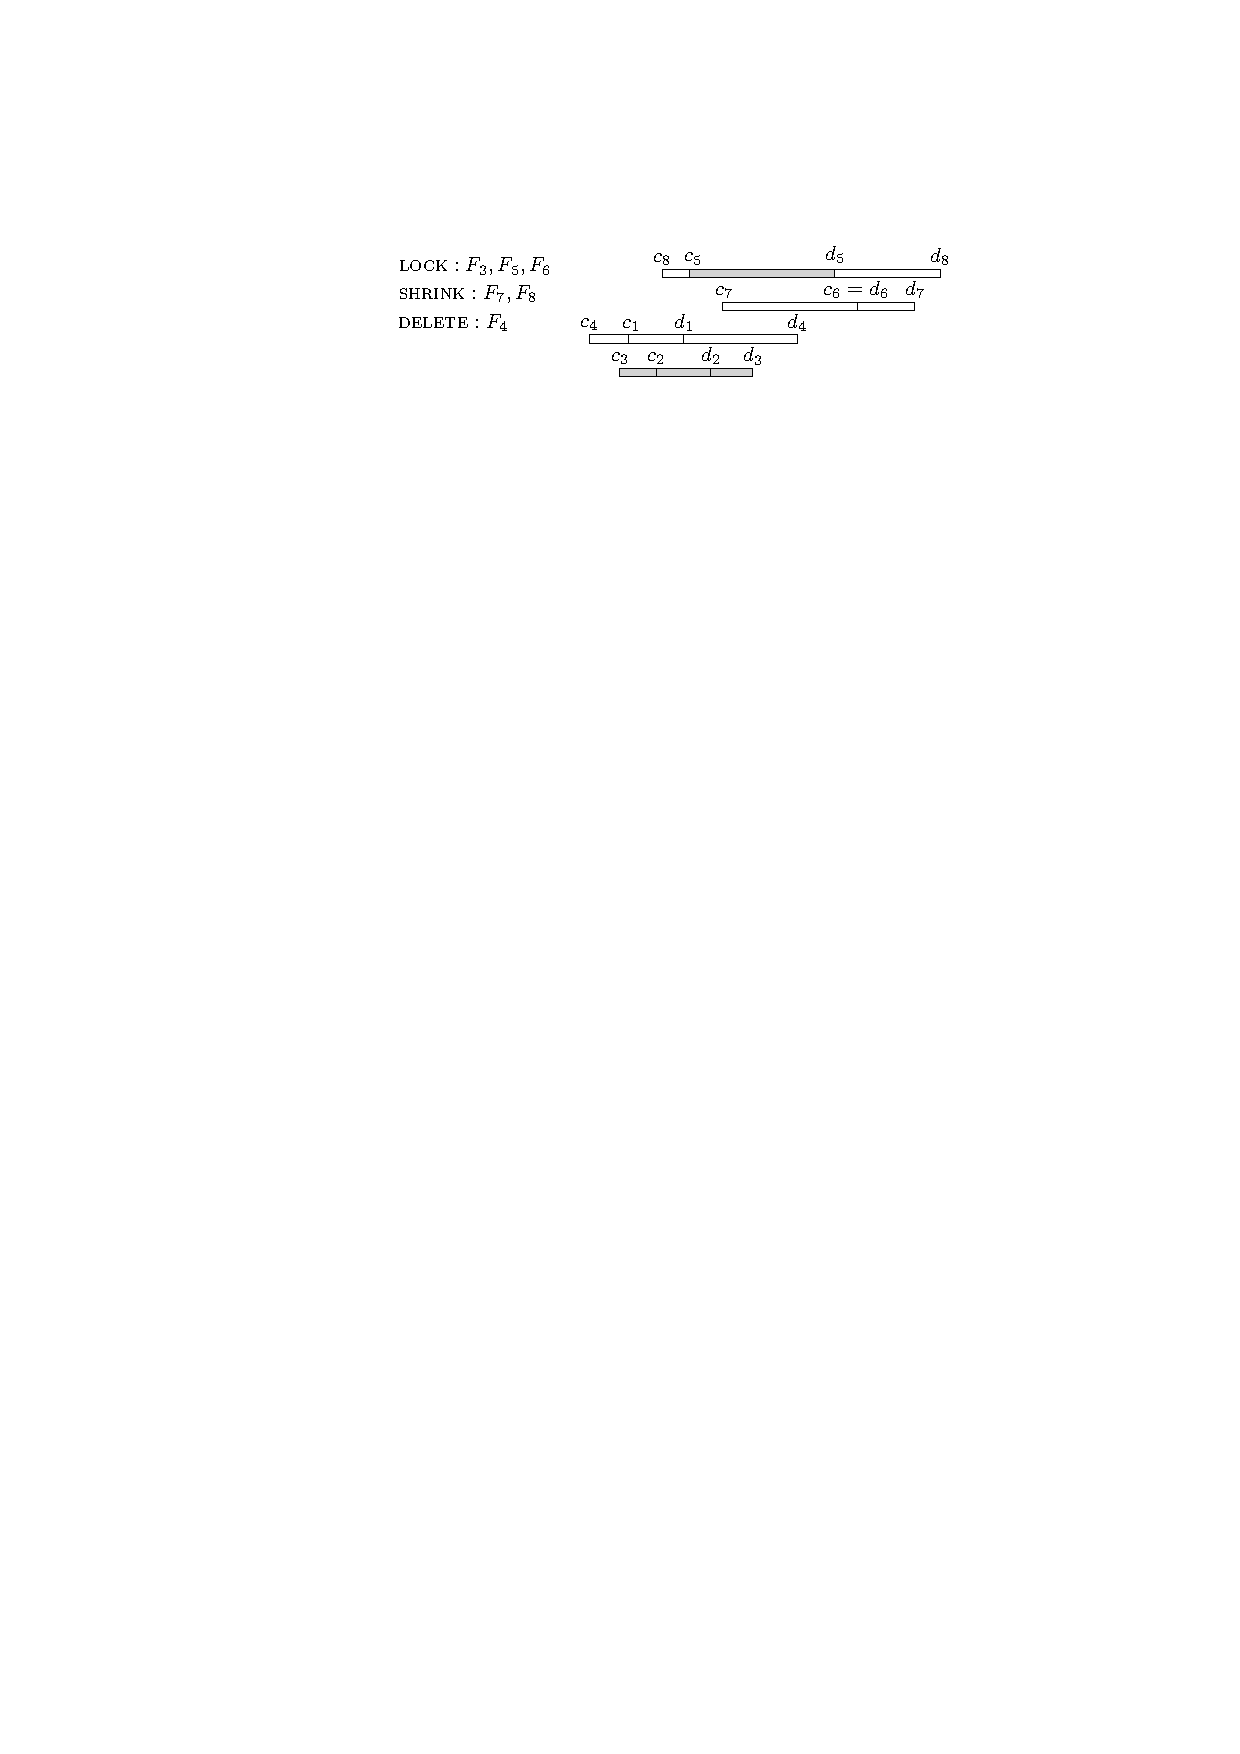
\includegraphics[scale=1]{chapter-3-interdiction/figure_ham_path}
\color{blue}
\begin{tabular}{cl|ccccc}
    && \multicolumn{5}{c}{memstate after action}\\
    $i$ & \ action & $\ell$ & $r$ & $k'$ & $\gamma$ & $\beta$ \\ 
    \hline
    %------
    - & \ initialize & $\infty$ & $\infty$ & 2 & 0 & 0 \\
    8 & \ 1b.) $\textsc{delay}(F_8)$ & $\infty$ & $\infty$ & 2 & 0 & 0\\
    7 & \ 1b.) $\textsc{delay}(F_7)$ & $\infty$ & $\infty$ & 2 & 0 & 0\\
    6 & \ 2c.) $\textsc{shrink}(F_7)$, $\textsc{lock}(F_6)$ & $\infty$ & $\infty$ & 1 & 1 & 1\\
    5 & \ 2c.) $\textsc{shrink}(F_8)$, $\textsc{lock}(F_5)$ & $c_5$ & $d_5$ & 0 & 2 & 2\\
    4 & \ 1b.) $\textsc{delay}(F_4)$ & $c_5$ & $d_5$ & 0 & 2 & 2\\
    3 & \ 1a.) $\textsc{lock}(F_3)$ & $c_3$ & $d_5$ & 0 & 2 & 2\\
    2 & \ 2a.) $\textsc{lock}(F_3)$, $\textsc{discard}(F_2)$ & $c_3$ & $d_5$ & 0 & 2 & 2\\
    1 & \ 2b.) $\textsc{delete}(F_4)$, $\textsc{discard}(F_1)$ & $c_3$ & $d_5$ & 0 & 2 & 1\\
\end{tabular}
\color{black}
\caption{An example execution of process $P$: The top half shows the intervals, where each pair of enveloping intervals represents an original interval and its corresponding replacement. The locked, shrunken, and deleted intervals are listed on the left. The \las{table} shows the memory states \las{$(i,\ell,r,k',\gamma,\beta)$} throughout the process.}
\label{fig:ham_path}
\end{figure}



\begin{lemma}
\label{lem:process_P}
(i) For every sequence of choices one can take in process $P$, there exists a candidate pair $(X,S)$, such that the final value of $\beta$ equals $s(X, S)$.

(ii) For all candidate pairs $(X,S)$, there is a sequence of choices one can take in process $P$, such that at the end of the process, $\beta \geq s(X, S)$. 
\end{lemma} 
\begin{proof}
(i) Firstly, observe that for any execution of $P$, the invariants \las{(\ref{eq:invariant_lock_in_alg})} are maintained throughout the process. \las{This is because the variable $L$ is only changed in the cases 1a.) and 2c.), each of which maintains the invariants. (If we have the special case $a'_t = b'_t$ in case 2c.), the variable $L$ remains unchanged.)}
Secondly, we claim that at the end of process $P$, for every $I \in \I$, exactly one of the keywords $\textsc{shrink}(I)$, $\textsc{delete}(I)$, or $\textsc{lock}(I)$ was called. 
Indeed, when we process the interval $I$, if \las{1b.)} $\textsc{ delay}(I)$ is called, then when we process the corresponding replacement interval $I'$, exactly one of the above operations is called for $I$.
\las{On the other hand, suppose 1a.) $\textsc{lock}(I)$} is called when we process the interval $I$. \las{We have to prove that we do not associate a conflicting keyword (i.e.\ a keyword other than $\textsc{lock}$) with $I'$.}
Indeed, by the design of the process, $I \subseteq L$ after this step.
Due to \las{invariants~(\ref{eq:invariant_lock_in_alg})} and the fact that \las{$I' \subseteq I$ and due to the constraints of cases 2a.), 2b.) and 2.c), we have the following: At a later iteration,} right before process $P$ considers interval $I'$, we still have $I' \subseteq I \subseteq L$. \las{Again, due to the constraints, at this point in time the options 2b.) and 2c.) are forbidden and option 2a.) is available.}
Hence, the option \las{2a.)} $\textsc{ lock}(I), \textsc{discard}(I')$ \las{is} called.

Now consider an execution of process $P$ such that $\beta_0$ is the final value of the variable $\beta$.
We define \las{$X \subseteq [n]$ ($S \subseteq [n]$ respectively)} as the set of the indices such that \textsc{shrink} (\textsc{delete} respectively) has been called for the corresponding intervals. 
By the observation above, we have $X \cap S = \emptyset$.
Further, whenever we call the operation $\textsc{shrink}$, $k'$ is decreased by 1.
As $k'$ starts at $k$ and cannot go below 0 during the process, we have $|X| \leq k$.
Hence, $(X, S)$ is a candidate pair.

Consider the set $R_0$ of all intervals $F \in \mathcal{F}$ that were locked during the execution of $P$. 
%For a connected component in $\graph{F_i}$ that corresponds to an empty interval $I'_t$ for some $t \in [n]$, the process should have taken the option $\textsc{shrink}(I_t)$, $\textsc{lock}(I'_t)$ at the relevant point, and $\beta$ is increased by one then.
It is easy to see that each connected component of $\graph(R_0)$ corresponds to exactly one \las{iteration} in the execution of $P$, where $\beta$ was increased and vice versa. 
Indeed, if the component corresponds to an empty interval $I'_t$, this  was the iteration $i$, for which $F_i = I'_t$.
Otherwise, using invariants (\ref{eq:invariant_lock_in_alg}), \las{this iteration occurs when the variable $r$ is re-assigned to the} rightmost point of the component of $\graph(R_0)$. 
Clearly, the amount of times $\beta$ was decreased is exactly $|S|$.
Further, whenever $\beta$ is increased, we also increase $\gamma$ subject to the cap of 2.
Hence, if $\gamma$ is less than 2 after the process, $c(\graph(R_0)) \leq  1$ and $\beta$ is set to $-\infty$. 
Overall, we have $\beta_0 = s(X, S)$. 

(ii) Consider the following execution of the process $P$.
For each $t \in [n]$, when considering $I_t$, we choose the option \las{1a.) }$\textsc{lock}(I_t)$ if $t \notin X \cup S$ and the option \las{1b.) } $\textsc{delay}(I_t)$ otherwise.
When considering $I'_t$, we choose \las{2a.) }$\textsc{lock}(I_t), \textsc{discard}(I'_t)$ if possible.
\las{What do we do when choosing 2a.) is impossible?}  \las{Consider the constraints on options 2a.), 2b.) and 2c.) For a similar reasoning as in the previous paragraph, the fact that 2a.) is impossible for $I'_t$ implies that for the same index $t$ we did not choose option 1a.) when encountering $I_t$.} This implies that $t \in X$ or $t \in S$.
Because $(X,S)$ is a candidate pair, it is impossible that $t \in X \cap S$.
Then we choose $\textsc{shrink}(I_t), \textsc{lock}(I'_t)$ if $t \in X$ and $\textsc{delete}(I_t),$ $\textsc{discard}(I'_t)$ if $t \in S$.

Following the argument for the proof of (i) above, we can construct $X'$ and $S'$ such that the final value $\beta$ of the execution of $P$ equals $s(X',S')$. 
By construction, $X' \subseteq X$ and $S' \subseteq S$.
Further, following the above execution of the process $P$, it is easy to see that the intervals on the real line corresponding to the connected components of $G_X - S$ are the same as those for $G_{X'} - S'$.
Therefore, $c(G_{X'} - S') - |S'| \geq c(G_{X} - S) - |S|$, and hence $s(X',S') \geq s(X,S)$.
The lemma then follows.
\qed
\end{proof}

\begin{lemma}
\label{lem:ham_path}
The maximum possible value of $\beta$ at the end of process $P$ can be computed in time $\bigO(kn^3)$ by reduction to the maximum-cost path in a DAG.
\end{lemma}
\begin{proof}
An instance of the maximum-cost path in a DAG problem is a tuple $(H, \omega)$, where $H$ is a DAG and a function $\omega: E(H) \to \R$ describes the edge cost of $H$.
The problem is to find a path in $H$ with the maximum cost, which is defined as the sum of edge costs along the path.
This problem can be solved with dynamic programming with runtime linear to the number of edges \las{and vertices} of $H$ \las{\cite{sedgewick2011algorithms}}.

We first construct an instance of this problem for the reduction. \las{Let $\mathcal{P} := \bigcup_{i=1}^{n}\set{a_i,b_i,a_i',b'_i}$.}
For every possible value assignments of $L = [\ell, r]$ (with \las{$\ell, r \in \mathcal{P}, \ell < r$}), every $k' \las{\in [k]}$, and $\gamma \in \set{1,2}$ describing the memory state of process $P$ at step $i \in \fromto{2n}{0}$, we add a vertex $(i,\ell,r,k',\gamma)$ in $H$. 
For $i \geq 1$, we create an edge from a vertex of the form $(i,\ell_1,r_1,k'_1,\gamma_1)$ to vertices $(i-1,\ell_2,r_2,k_2',\gamma_2)$, if and only if there is some possible choice in $P$ such that if the current memory state is $(i,\ell_1,r_1,k'_1,\gamma_1)$ then the new memory state would be $(i-1, \ell_2, r_2, k_2',\gamma_2)$ after this choice. 
Observe that the knowledge of $(i, \ell_1, r_1, k'_1,\gamma_1)$ suffices to determine which \las{of the choices 1a.), 1b.), 2a.) 2b.) and 2c.)} are possible and to determine the new memory state \las{(note that the interval $F_i$ can be derived from $i$)}. 
The edge costs are given by $+1$, if the line $\beta \leftarrow \beta + 1$ is called, by $-1$, if the line $\beta \leftarrow \beta- 1$ is called.
One exception is the step from a vertex $(1,\ell_1,r_1,k'_1,\gamma_1)$ to a vertex $(0,\ell_2,r_2,k'_2,\gamma_2)$, where $\gamma_2 < 2$.
In this case, we set the corresponding edge cost to $-\infty$.
The costs of all other edges are 0.

By construction, $H$ is a DAG, because for any edge in $H$, the first index of the starting vertex is higher than that of the ending vertex.
\las{Consider} a path connecting the starting vertex $(2n, \infty, \infty, k, 0)$ to a vertex $(0, \ell, r, k', \gamma)$. \las{By definition}, its cost is the final value \las{of} $\beta$ at the end \las{of} the execution of $P$ \las{which corresponds to that path}.
Consequently, the cost of the maximum-cost path is exactly the maximum possibe value of $\beta$ at the end of process $P$. 
There are $\bigO(n)$ possible values for each of $i, \ell, r$ respectively, so $H$ has $\bigO(kn^3)$ vertices and edges. Hence the desired path can be found in $\bigO(kn^3)$ time.
\qed
\end{proof}

\paragraph*{Proof of Theorem~\ref{thm:ham}(a).}
Let $\beta_{\max}$ be the maximum possible value of $\beta$ at the end of process $P$.
As a consequence of Lemma~\ref{lem:process_P}, there exists a candidate pair $(X,S)$ such that $s(X,S) = \beta_{\max}$, and
for any candidate pair $(X',S')$, there exists an execution of $P$ such that the final value of $\beta$ is at least $s(X',S')$.
This implies that $\beta_{\max}$ is the maximum of $s(X,S)$ over all candidate pairs $(X,S)$, i.e., the value of the original problem that we want to compute.
By Lemma~\ref{lem:ham_path}, $\beta_{\max}$ can be computed in time $\bigO(kn^3)$.
Theorem~\ref{thm:ham}(a) then follows.
\qed

\subsection{Interdiction Problems for Hamiltonicity}
\label{subsection:ham_interdict}

In the interdiction problem for Hamilton path (cycle), we are given shrinking intervals $\I, \I'$, such that $\graph(\I)$ has a Hamilton path (cycle), and the interdictor wishes to select $X \subseteq [n]$ of size at most $k$, such that $\graph(\I_X)$ does not have a Hamilton path (cycle) anymore.
Similarly in the interdiction problem for path cover, we also have shrinking intervals, and the objective of the interdictor is to maximize the size of the path cover within the budget $k$ shrinkages.

\paragraph*{Proof of Theorem~\ref{thm:ham}(b)-(d).}
These are implied by Theorem~\ref{thm:scat} and Theorem~\ref{thm:ham}(a).
To solve these problems, we first compute $\max_{|X| \leq k}\scat(G_X)$, i.e. the value of the assistance problem of the scattering number.
This value is also the value for the interdiction problem for path cover.
For the interdiction problems for Hamilton path and Hamilton cycle, we can conclude that the interdictor can interdict successfully, if and only if this value is more than 1 and 0 respectively.
Therefore, these problems can also be solved in time $\bigO(kn^3)$.
\qed

\subsection{Most Vital Nodes Problem for Hamiltonicity}
\label{subsection:ham_mvn}
\las{In the most vital nodes problem for Hamilton path (cycle, respectively), we are given an interval graph, which has a Hamilton path (cycle, respectively) and a budget $k$. The question is whether the interdictor can destroy the property that the graph has a Hamilton path (cycle) by deleting at most $k$ vertices. More generally, the most vital nodes problem for path cover is to compute the number $\max_{X \subseteq V, |X| \leq k} \text{pc}(G - X)$, where $\text{pc}$ denotes the path cover number. We show that all these problems can be solved in polynomial time.}

Similar to other graph parameters discussed in this paper, a natural question is whether the most vital nodes problems for Hamilton path, Hamilton cycle, and path cover are special cases of the shrink-expand framework.
The simple answer is no.
Here, shrinking to an empty interval and deleting a vertex yield different effect.
The former operation creates an isolated vertex and disconnects the graph, while the latter does not necessarily make the graph non-hamiltonian.

However, the most vital nodes problems for the above parameters can be reduced to the assistance problem for scattering number.
By Theorem~\ref{thm:scat}, the former problems can be immediately solved, if we know the value of the following problem $\textsc{Scat}(G,k)$: Given an interval graph $G$ and a budget $k$, what is the maximum scattering number that can be achieved after $k$ vertex \las{deletions}?
Note that this is technically not a most vital nodes problem in the traditional sense, as the goal of two players are aligned instead of conflicting.
The value of the problem $\textsc{Scat}(G,k)$ above in turn can be easily derived from the assitance problem for scattering number, as shown in the following lemma.

\begin{lemma}
Let $G$ be an interval graph and $k$ an integer.
Let $s_1$ be the value of the problem $\textsc{Scat}(G,k)$.
Let $s_2$ be the value of the assistance problem for scattering number with the budget $k$, where the original intervals are the intervals of $G$, and the replacement intervals are all empty intervals.
Then $s_1 = s_2 - k$.
\end{lemma}
\begin{proof}
Consider an optimal solution of $\textsc{Scat}(G,k)$.
There are $k' \leq k$ deleted vertices in this solution.
Replacing these vertices with empty intervals in the assistance problem yields a valid (but not necessarily optimal) solution with value $s_1 + k'$.
Since shrinking an interval always strictly increases the value of the scattering number, we shrink further $k - k'$ other intervals.
The value then becomes $s_1 + k$ and this is still a valid solution.
Hence, $s_1 + k \leq s_2$.

For the other direction, with the same observation that shrinking intervals always make the value better, there must exist an optimal solution of the assistance problem with exactly $k$ \las{shrunken} intervals.
We then delete these intervals in the problem $\textsc{Scat}(G,k)$, yielding a valid (but not necessarily optimal) solution with value $s_2 - k$.
Hence, $s_1 \geq s_2 - k$.

The lemma then follows. 
\qed
\end{proof}

Combining the above lemma with Theorem~\ref{thm:ham}(a), we obtain the following:
\begin{corollary}
The most vital nodes problem \las{on interval graphs} for Hamilton path, Hamilton cycle, and path cover can be solved in time $\bigO(kn^3)$
\end{corollary}

\subsection{Graph Toughness}
\label{subsection:tough}
In this subsection, we will briefly discuss a related parameter, graph toughness, which was introduced by Chv\'{a}tal~\cite{Chvatal1973} as a measure of graph connectivity. 
A graph $G$ is $t$-tough if $|S| \geq t \cdot c(G - S)$ for any cutset $S$, i.e., $S \subseteq V(G)$ and $c(G - S) > 1$.
In the interdiction problem for graph toughness, we are given shrinking intervals $\I, \I'$, such that $G(\I)$ is $t$-tough, and the interdictor wishes to select $X \subseteq \I$ of size at most $k$, such that $G(\I_X)$ is not $t$-tough, i.e., we have
\[
	\max \{t \cdot c(G_X - S) - |S|  : S \subseteq \I_X \text{ and } c(G_X - S) > 1 \} > 0.
\]

If the set on the left-hand side is empty, then the graph $G_X$ is a complete graph and we define the maximum to be $-\infty$.

Observe that the left-hand side of the above expression is almost identical to the definition of scattering number, except for the factor $t$ in front of $c(G_X - S)$.
Therefore, we can adapt the method to solve the assistance problem for scattering number to solve this problem.
In fact, the only modification to the process $P$ is to replace all instances of $\beta \leftarrow \beta + 1$ by $\beta \leftarrow \beta + t$.
Effectively, each component now contributes $t$ instead of 1 toward the final sum.
Hence, following a completely analogous proof to the proof of Theorem~\ref{thm:ham}(a), we obtain the following:

\begin{corollary}
In the shrink-expand framework, the interdiction problem for graph toughness can be solved in time $\bigO(kn^3)$.
\end{corollary}
